\item O ônibus espacial está localizado no ``espaço profundo'', onde os efeitos da gravidade podem ser
desprezados. Ele tem uma massa de \SI{120}{\mega\gram}, um centro de massa em $G$ e um raio de giração $(k_{G})_{x}=\SI{14}{\meter}$ em relação ao eixo $x$. Ele está originalmente se deslocando para frente a $v=\SI{3}{\kilo\meter/\second}$ quando o piloto liga o motor em $A$, criando um empuxo $T=600(1-e^{-0.3t})\,\SI{}{\kilo\newton}$, onde $t$ é dado em segundos. Determine a velocidade angular do ônibus espacial \SI{2}{\second} mais tarde.

\import{../answers}{answer-2}

\vspace{-.5cm}
\begin{flushright}
	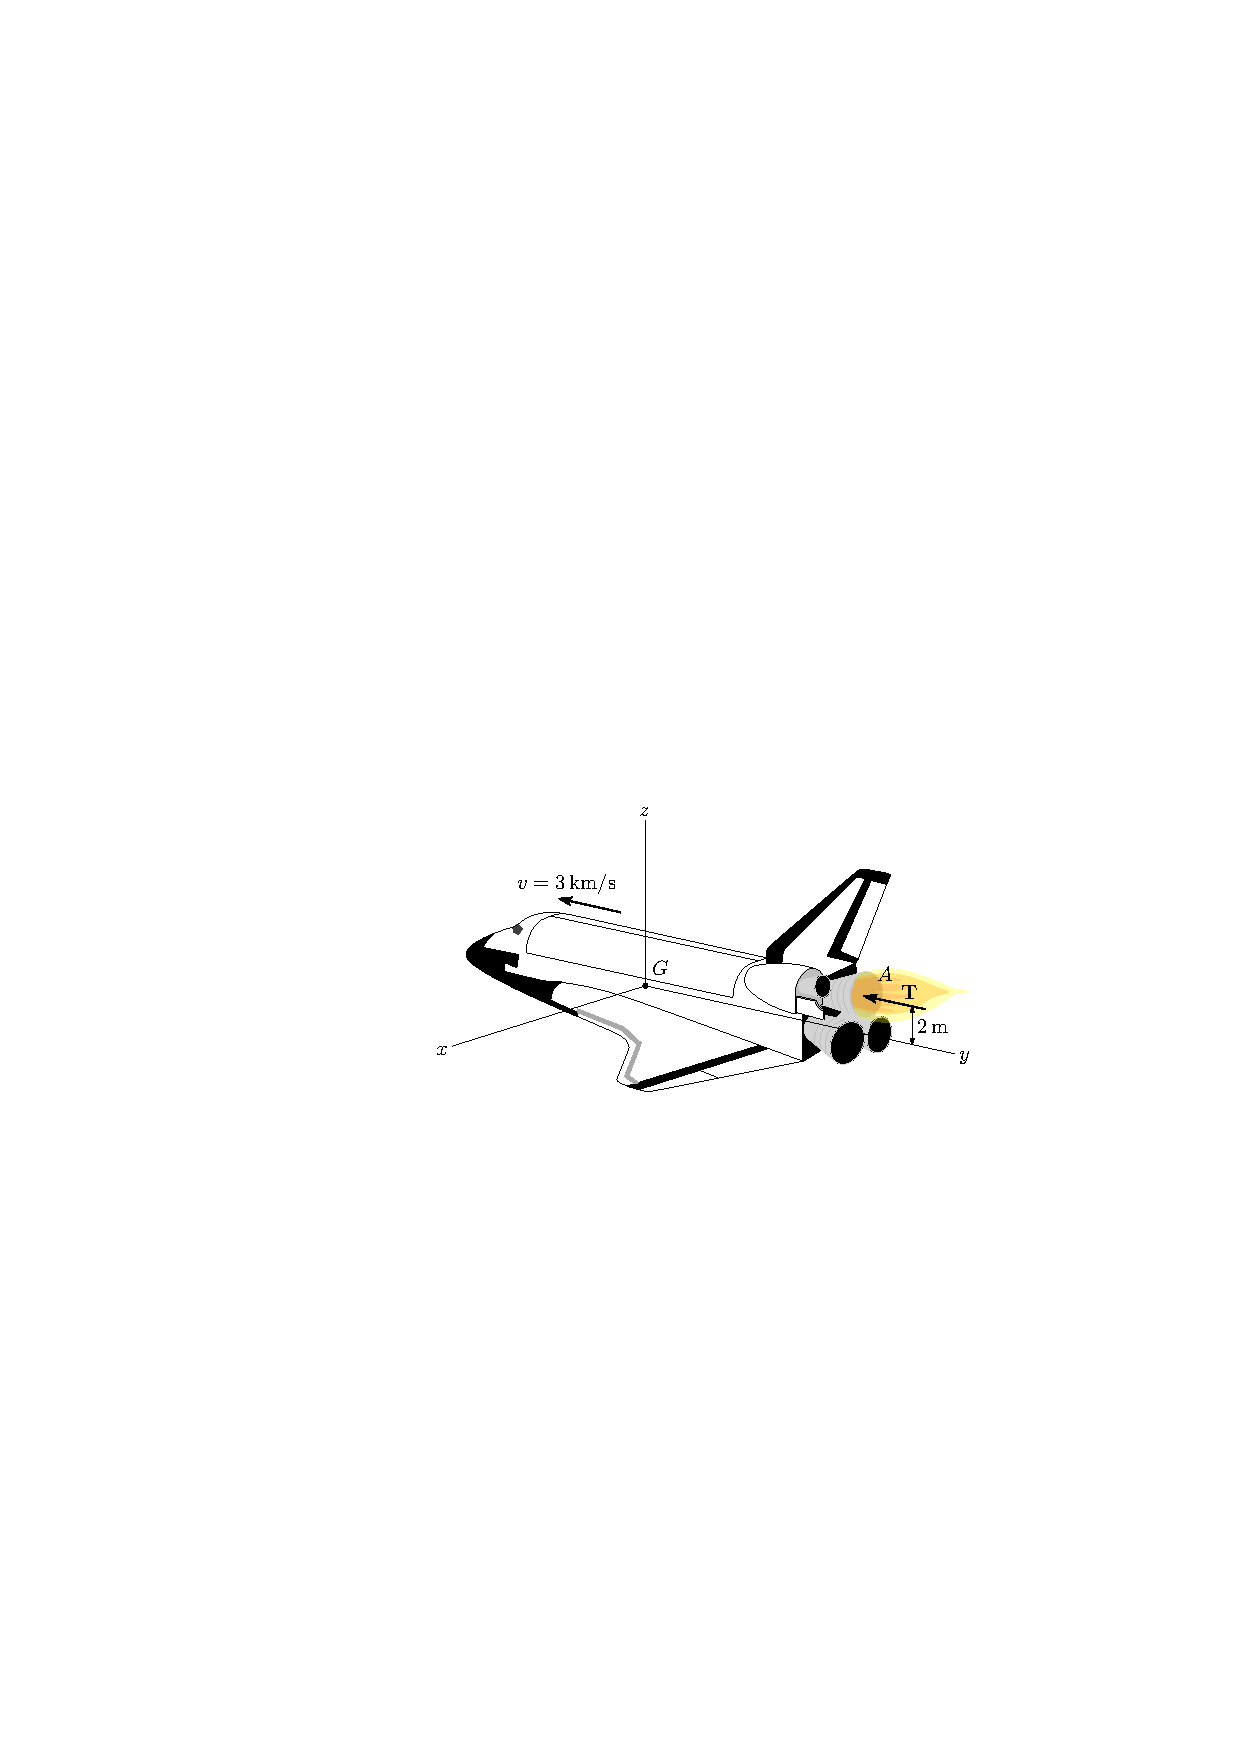
\includegraphics[scale=1.3]{../../images/draw_1}
\end{flushright}